\vspace{-0.2cm}
\section{Experiments}
\label{sec:experiments}
\vspace{-0.15cm}
We use AgentJudgeBench to evaluate the extent to which LLM-judge alignment depends on the generator, query difficulty, and ground-truth availability. Protocol details (prompts, scoring, conditions) are in Section~\ref{sec:methodology}; model identifiers are in Appendix~\ref{app:generators} and Appendix~\ref{app:judges}.

\subsection{Experimental Setup}
\label{sec:exp:design}
We instantiate a fully-crossed factorial over three factors: generator $g \in \mathcal{G}$ (five models, 3B to frontier), judge $j \in \mathcal{J}$ (six LLMs), and difficulty $d \in \{\text{easy}, \text{medium}, \text{hard}\}$. Each cell is observed under both with GT and without GT conditions, yielding 90 factorial cells and $321{,}648$ valid (generator, judge, difficulty, record) tuples. Exact per-cell counts are in Appendix~\ref{app:eval-stats}. We report $\mathrm{align}(j, g, d, c)$ (Eq.~\ref{eq:alignment}) and, where relevant, GT lift (Eq.~\ref{eq:lift}).

\subsection{Results and Analysis}
\label{sec:exp:main}
Table~\ref{tab:full-results} reports every configuration in the factorial design. Each generator occupies a sub-block with six rows corresponding to the judges in $\mathcal{J}$, plus a seventh row for Prometheus-2~\citep{kim2024prometheus2}, a judge-specialised model added as a baseline across all five generators and both GT conditions (Limitations), shown for reference and excluded from the six-judge statistics below. Columns pair each difficulty level with its with-GT and without-GT conditions; bold entries mark the highest alignment within each (difficulty, condition) column of each sub-block.

\textbf{Finding 1: Monotone difficulty degradation.} All 30 (generator, judge) pairs exhibit strictly monotone alignment degradation from easy to hard under both conditions (Table~\ref{tab:full-results}), without-GT degradation roughly $1.5\times$ larger than with-GT. On hard without-GT records, all six judges converge to a narrow $77$--$82\%$ band across four of five generators (including frontier GPT-5.4), indicating a task-level rather than judge-level ceiling; degradation curves are in Appendix~\ref{app:degradation}.
\begin{table}[h]
\centering
\small
\setlength{\tabcolsep}{3pt}
\renewcommand{\arraystretch}{1.02}

\resizebox{\columnwidth}{!}{%
\begin{tabular}{llrrrrr}
\toprule

\textbf{Judge} &
\textbf{Diff} &
\textbf{GT} &
\textbf{withoutGT} &
\textbf{cGT} &
\textbf{$\Delta_{\text{cGT-GT}}$} &
\textbf{$\Delta_{\text{cGT-noGT}}$} \\

\midrule

\multirow{3}{*}{QwQ-32B}
& Easy   & 96.6 & 95.6 & 95.5 & $-1.1$ & $-0.1$ \\
& Medium & 92.3 & 92.0 & 92.0 & $-0.3$ & $0.0$ \\
& Hard   & 84.6 & 84.4 & 84.6 & $0.0$ & $+0.2$ \\

\addlinespace[2pt]

\multirow{3}{*}{Gemini}
& Easy   & 90.7 & 95.7 & 92.5 & $+1.8$ & $-3.2$ \\
& Medium & 86.4 & 92.1 & 86.4 & $0.0$ & $-5.7$ \\
& Hard   & 78.9 & 84.6 & 78.9 & $0.0$ & $-5.7$ \\

\bottomrule
\end{tabular}%
}
\vspace{-0.1cm}
\caption{Full C3 results on Llama-3.3-70B generator. All values are mean alignment (\%) over 3,764--3,771 records per cell.
\textbf{cGT}: corrupted-GT condition. \textbf{Gemini}: Gemini 2.5 Pro.
\textbf{$\Delta_{\text{cGT-GT}}$}: corrupted-GT minus standard GT.
\textbf{$\Delta_{\text{cGT-noGT}}$}: corrupted-GT minus without GT.}
\vspace{-0.2cm}
\label{tab:c3-anchoring}

\end{table}
\textbf{Scope of Finding 1.} The medium$\to$hard drop (${\approx}5$--$7$\,pp with GT) is the primary evidence for difficulty-driven degradation; hard rewrites are unanimously validated on $93.9\%$ of records (Appendix~\ref{app:rewrite-validation}), while the easy$\to$medium step (unanimous on $58.1\%$) partially reflects paraphrase-robustness.

\textbf{Finding 2: Ground-truth exposure is not monotonically beneficial.} GT lift (Eq.~\ref{eq:lift}) is positive for QwQ-32B and GPT-OSS-120B, but negative for GPT-5.4 and Gemini-2.5-Pro (non-overlapping bootstrap CIs; Appendix~\ref{app:bootstrap-ci}). Figure~\ref{fig:permetric} shows the effect concentrates in sequence accuracy: frontier judges anchor to the GT trace's ordering and penalise functionally equivalent but structurally deviant sequences (case studies in Appendix~\ref{app:anchoring-cases}).
\begin{table}[t]
\centering

\small
\setlength{\tabcolsep}{2.4pt}
\renewcommand{\arraystretch}{0.80}

\begin{tabular*}{\columnwidth}{@{\extracolsep{\fill}}llcccccc}

\toprule

& &
\multicolumn{2}{c}{\scriptsize\textbf{Easy}} &
\multicolumn{2}{c}{\scriptsize\textbf{Med.}} &
\multicolumn{2}{c}{\scriptsize\textbf{Hard}} \\

\cmidrule(lr){3-4}
\cmidrule(lr){5-6}
\cmidrule(lr){7-8}

\scriptsize\textbf{Gen.} &
\scriptsize\textbf{Judge} &
\scriptsize\textbf{GT} &
\scriptsize\textbf{No GT} &
\scriptsize\textbf{GT} &
\scriptsize\textbf{No GT} &
\scriptsize\textbf{GT} &
\scriptsize\textbf{No GT} \\

\midrule

\multirow{7}{*}{\rotatebox{90}{\scriptsize\textit{Sm3B}}}
& OSS20  & 84.8 & 85.3 & 81.7 & 79.3 & 77.4 & 69.0 \\
& QwQ32  & \textbf{90.0} & 86.7 & \textbf{84.8} & 80.3 & 77.2 & 69.7 \\
& OSS120 & 89.2 & 86.3 & \textbf{84.8} & 80.2 & \textbf{77.8} & 69.7 \\
& ClS4   & 86.5 & 86.8 & 81.3 & 80.9 & 74.2 & 71.2 \\
& Gem    & 81.1 & 86.6 & 77.7 & 80.7 & 73.4 & 70.8 \\
& GPT5   & 86.0 & \textbf{87.3} & 81.6 & \textbf{82.0} & 76.9 & \textbf{73.3} \\
& Prom2  & 64.0 & 67.1 & 61.6 & 64.9 & 58.6 & 60.2 \\

\midrule

\multirow{7}{*}{\rotatebox{90}{\scriptsize\textit{Ll8B}}}
& OSS20  & 87.4 & 89.5 & 85.3 & 85.7 & 81.2 & 75.9 \\
& QwQ32  & \textbf{94.2} & 91.2 & \textbf{90.8} & 86.8 & \textbf{84.1} & 76.6 \\
& OSS120 & 93.1 & 90.7 & 89.8 & 86.6 & 83.6 & 76.6 \\
& ClS4   & 90.3 & 90.6 & 86.5 & 86.6 & 80.3 & 77.1 \\
& Gem    & 85.9 & \textbf{91.9} & 83.3 & \textbf{87.6} & 78.7 & 78.2 \\
& GPT5   & 88.5 & 91.4 & 85.0 & 87.5 & 80.6 & \textbf{79.0} \\
& Prom2  & 60.8 & 63.2 & 59.0 & 60.8 & 56.7 & 58.4 \\

\midrule

\multirow{7}{*}{\rotatebox{90}{\scriptsize\textit{Qw32B}}}
& OSS20  & 88.4 & 93.2 & 85.8 & 88.7 & 82.7 & 81.1 \\
& QwQ32  & \textbf{95.0} & 93.9 & \textbf{90.9} & 89.1 & \textbf{84.7} & 81.1 \\
& OSS120 & 93.9 & 94.0 & 90.0 & 89.2 & 84.4 & 81.3 \\
& ClS4   & 92.7 & 94.0 & 88.5 & 89.2 & 82.1 & 81.6 \\
& Gem    & 86.4 & \textbf{94.1} & 83.0 & 89.2 & 78.1 & 81.4 \\
& GPT5   & 90.5 & 93.9 & 86.4 & \textbf{89.4} & 81.9 & \textbf{81.7} \\
& Prom2  & 64.4 & 66.7 & 62.0 & 64.5 & 59.1 & 61.5 \\

\midrule

\multirow{7}{*}{\rotatebox{90}{\scriptsize\textit{Ll70B}}}
& OSS20  & 89.0 & 94.5 & 87.2 & 91.2 & 83.9 & 84.0 \\
& QwQ32  & \textbf{96.6} & 95.6 & \textbf{93.6} & 92.1 & \textbf{87.5} & 84.4 \\
& OSS120 & 96.0 & 95.5 & 93.0 & 92.1 & 87.2 & 84.5 \\
& ClS4   & 93.3 & 94.6 & 89.9 & 90.7 & 83.7 & 83.3 \\
& Gem    & 90.5 & \textbf{95.7} & 86.5 & \textbf{92.2} & 82.2 & \textbf{84.6} \\
& GPT5   & 91.4 & 95.2 & 87.4 & 91.7 & 83.0 & \textbf{84.6} \\
& Prom2  & 66.5 & 68.6 & 62.8 & 65.2 & 58.3 & 60.2 \\

\midrule

\multirow{7}{*}{\rotatebox{90}{\scriptsize\textit{GPT5}}}
& OSS20  & 83.1 & 85.6 & 82.1 & 83.9 & 79.4 & 79.5 \\
& QwQ32  & 85.7 & 85.8 & 84.3 & 84.2 & 80.5 & 79.8 \\
& OSS120 & 84.8 & 85.3 & 83.9 & 83.3 & 80.7 & 78.6 \\
& ClS4   & \textbf{86.1} & \textbf{87.3} & \textbf{84.5} & \textbf{85.4} & 80.7 & \textbf{81.2} \\
& Gem    & 81.6 & 85.2 & 80.2 & 83.3 & 77.6 & 78.4 \\
& GPT5   & 85.8 & 87.0 & 84.1 & 84.9 & \textbf{81.4} & 79.8 \\
& Prom2  & 57.1 & 60.9 & 57.9 & 61.1 & 57.8 & 60.5 \\

\bottomrule
\end{tabular*}
\vspace{-0.2cm}
\caption{LLM--judge alignment (\%) with the programmatic reference across generators, judges, difficulty, and GT condition. Bold = column-wise maximum within each generator block among the six main judges. Prom2 = Prometheus-2, a judge-specialised baseline (Limitations); shown for reference and not counted toward bold column-wise maxima or six-judge statistics.}
\label{tab:full-results}
\vspace{-0.7cm}
\end{table}
\textbf{C3 control.} Replacing the reference with a wrong GT from a different record confirms pure anchoring (Table~\ref{tab:c3-anchoring}): Gemini-2.5-Pro aligns identically under standard and corrupted GT, while QwQ-32B tracks without-GT within $0.2$\,pp. Full results are in Appendix~\ref{app:c3-table}.
\begin{figure*}[t]
\centering
  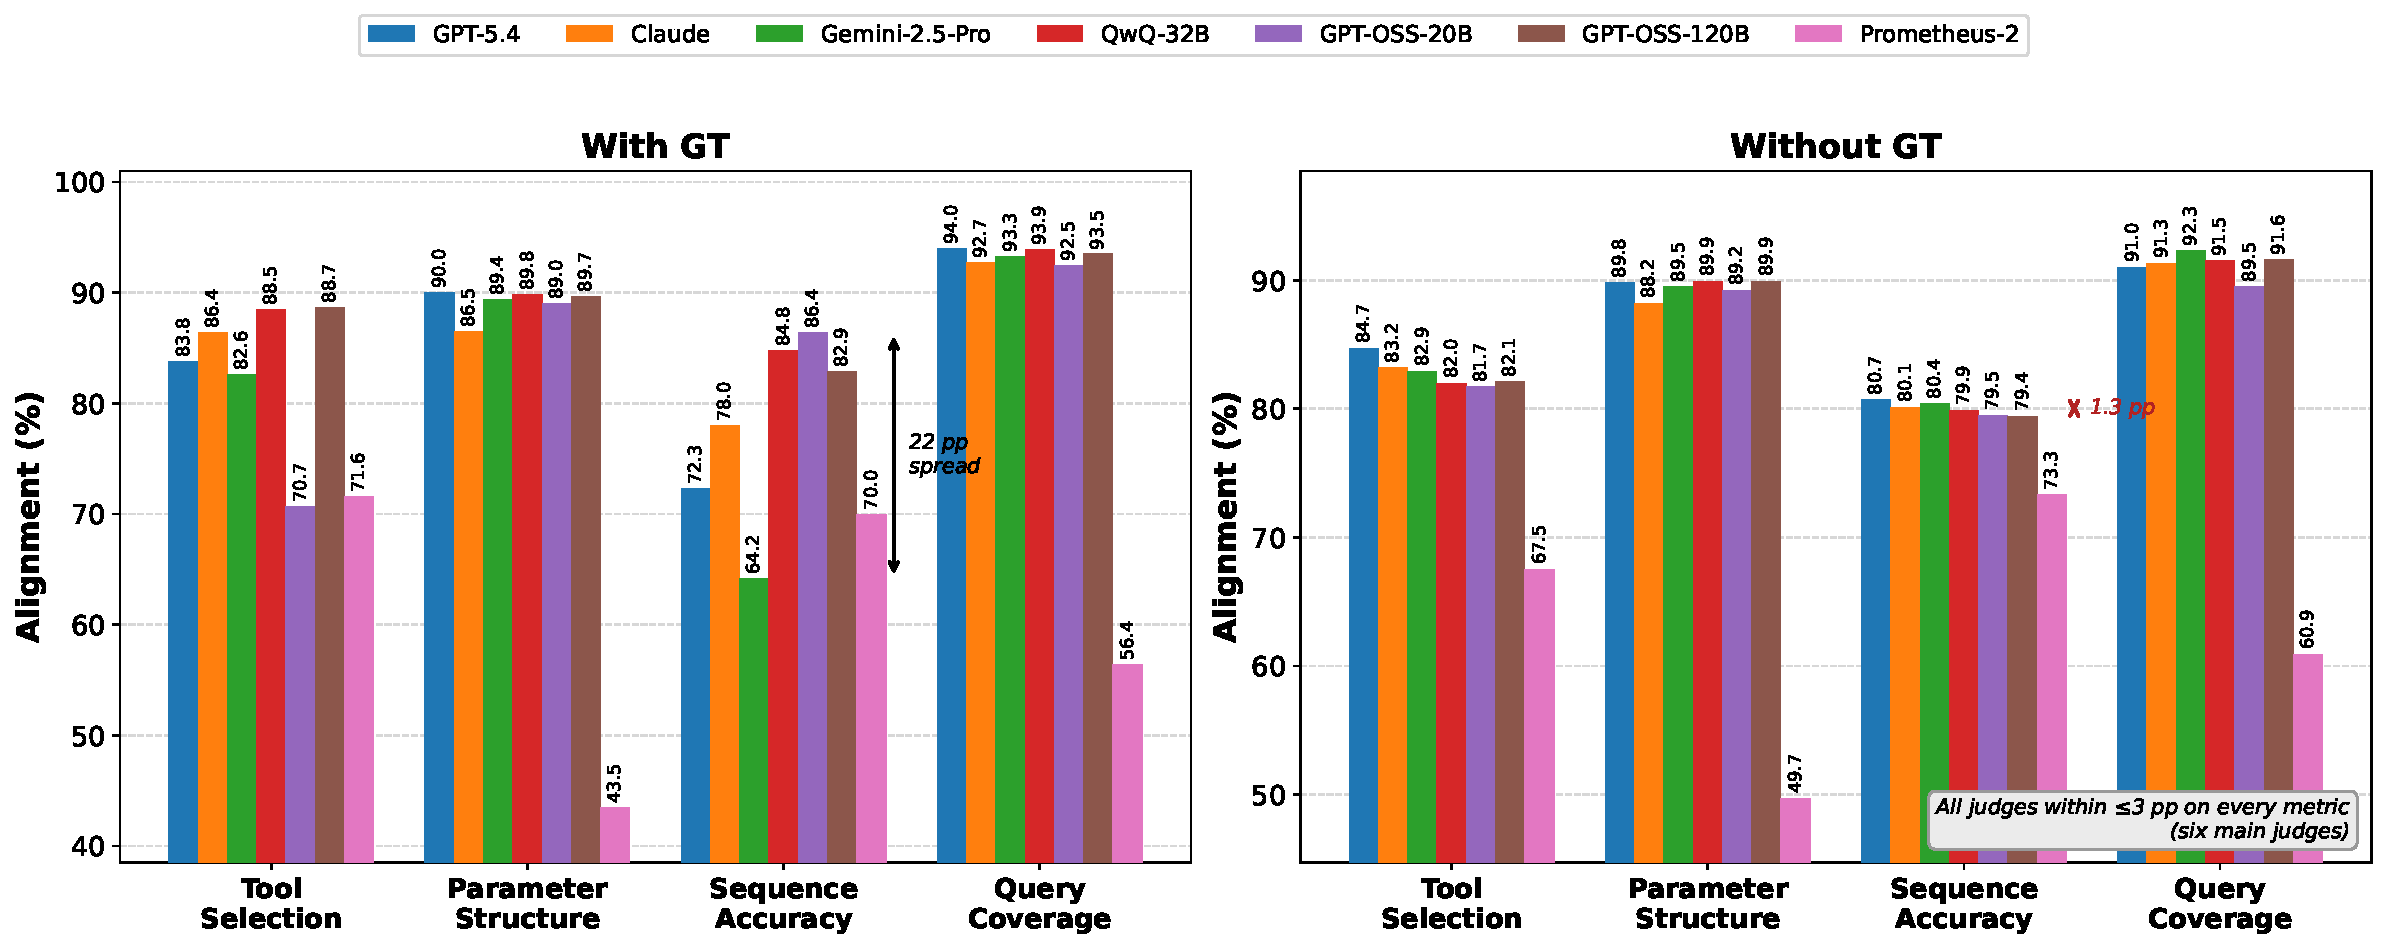
\includegraphics[width=0.85\textwidth]{figures/per_metric_both.pdf}
  \vspace{-0.2cm}
  \caption{Per-metric alignment (with and without GT) across the six main judges, plus Prometheus-2 (judge-specialised baseline; Limitations), shown for reference.}
  \label{fig:permetric}
  \vspace{-0.5cm}
\end{figure*}
\footnotetext{Cohen's $\kappa$ measures inter-rater agreement corrected for chance: ($0$=chance, $1$=perfect; $0.2$--$0.4$ ``fair,'' $0.4$--$0.6$ ``moderate,'' ${\geq}0.6$ ``substantial'') agreement. All $\kappa$ values here fall in the fair-to-substantial range ($0.225$--$0.606$), consistent with the structural complexity of the four-metric scoring task.}
\textbf{Finding 3: Best judge depends on configuration.} QwQ-32B leads GT alignment in 10 of 15 (generator, difficulty) cells but is never the top without-GT judge; Gemini-2.5-Pro and GPT-5.4 lead without-GT on stronger and weaker generators, respectively. See Appendix~\ref{app:decision-guide} for a deployment decision table. The following research questions explain the mechanisms behind Findings 1--3.

\textbf{RQ1: Which metrics and DAG topologies are hardest for judges?}
\label{sec:exp:disaggregation}

Figure~\ref{fig:permetric} breaks alignment into per-metric components: with GT, sequence accuracy is the weakest dimension with substantial inter-judge spread, while without GT all judges compress to a narrow band, reflecting the $1.0$-default rubric. DAG topology imposes a judge-independent difficulty ordering (\emph{fan-out} easiest, \emph{loop-like}/\emph{fan-in} hardest); full breakdowns are in Appendices~\ref{app:permetric-table}--\ref{app:pertopology-table}.

\textbf{RQ2: How much do judges agree with each other?}
\label{sec:exp:interjudge}

Table~\ref{tab:interjudge} reports pairwise judge agreement. Mean agreement is $79.1\%$ ($\kappa=0.419$) with GT and $92.6\%$ ($\kappa=0.559$) without GT; the higher without-GT value reflects prompt-driven verdict compression rather than genuine consensus. The highest agreement is QwQ-32B$\times$GPT-OSS-120B ($89.4\%$, $\kappa=0.606$), and the lowest is Claude Sonnet 4.5$\times$GPT-OSS-20B ($70.4\%$, $\kappa=0.225$). Under without-GT, pairwise $\kappa$ decreases monotonically with judge tier separation ($\rho=-0.825$\footnote{Spearman's $\rho$ measures the rank correlation between the pairwise judge tier gap (by parameter count) and their $\kappa$ agreement score; $|\rho|>0.7$ indicates a strong monotone relation.}, $p<0.01$); this relationship vanishes under GT ($\rho=-0.171$), where GT acts as a shared anchor. Disagreement concentrates at the $0.5$ partial-credit boundary ($94$--$97\%$ of off-diagonal entries); verdict-level confusion matrices are in Appendix~\ref{app:confusion} and a binary scale ablation is in Appendix~\ref{app:abl-binary}. Prometheus-2 agrees with every judge at close to chance level under both conditions ($42$--$52\%$ exact, $\kappa = 0.01$--$0.07$; Table~\ref{tab:interjudge}), well below the fair-to-substantial range spanned by the six main judges, indicating it forms its own bloc rather than a lower-alignment member of the general-purpose cluster (Limitations).

\begin{table}[t]
\centering
\small
\setlength{\tabcolsep}{3.5pt}
\renewcommand{\arraystretch}{1.02}

\resizebox{\columnwidth}{!}{%
\begin{tabular}{lccccccc}
\toprule

& \textbf{OSS-20B}
& \textbf{QwQ-32B}
& \textbf{OSS-120B}
& \textbf{Claude S. 4.5}
& \textbf{Gemini}
& \textbf{GPT-5.4}
& \textbf{Prom2} \\

\midrule

OSS-20B
& {-}
& \cellcolor{blue!8}77.4
& \cellcolor{blue!8}78.4
& \cellcolor{blue!8}70.4
& \cellcolor{blue!8}74.5
& \cellcolor{blue!8}75.2
& \cellcolor{blue!8}42.2 \\

QwQ-32B
& \cellcolor{orange!15}0.386
& {-}
& \cellcolor{blue!8}\textbf{89.4}
& \cellcolor{blue!8}85.1
& \cellcolor{blue!8}80.7
& \cellcolor{blue!8}79.7
& \cellcolor{blue!8}49.0 \\

OSS-120B
& \cellcolor{orange!15}0.414
& \cellcolor{orange!15}\textbf{0.606}
& {-}
& \cellcolor{blue!8}83.2
& \cellcolor{blue!8}81.6
& \cellcolor{blue!8}79.8
& \cellcolor{blue!8}48.0 \\

Claude S. 4.5
& \cellcolor{orange!15}0.225
& \cellcolor{orange!15}0.490
& \cellcolor{orange!15}0.424
& {-}
& \cellcolor{blue!8}76.5
& \cellcolor{blue!8}78.4
& \cellcolor{blue!8}47.4 \\

Gemini
& \cellcolor{orange!15}0.387
& \cellcolor{orange!15}0.411
& \cellcolor{orange!15}0.437
& \cellcolor{orange!15}0.328
& {-}
& \cellcolor{blue!8}76.4
& \cellcolor{blue!8}44.1 \\

GPT-5.4
& \cellcolor{orange!15}0.419
& \cellcolor{orange!15}0.446
& \cellcolor{orange!15}0.449
& \cellcolor{orange!15}0.430
& \cellcolor{orange!15}0.432
& {-}
& \cellcolor{blue!8}42.6 \\

Prom2
& \cellcolor{orange!15}0.026
& \cellcolor{orange!15}0.074
& \cellcolor{orange!15}0.055
& \cellcolor{orange!15}0.062
& \cellcolor{orange!15}0.009
& \cellcolor{orange!15}0.036
& {-} \\

\bottomrule
\end{tabular}%
}
\vspace{-0.2cm}
\caption{Pairwise inter-judge agreement under the with GT condition.
\colorbox{blue!12}{\strut Upper triangle}: exact metric-level agreement (\%);
\colorbox{orange!20}{\strut Lower triangle}: Cohen's $\kappa$\protect\footnotemark. Prom2 (Prometheus-2, judge-specialised baseline) row/column added for reference; excluded from the six-judge mean agreement statistics discussed in the text.}
\label{tab:interjudge}
\vspace{-0.3cm}
\end{table}

A soft jury of all six judges matches but does not exceed the top individual judge ($82.5\%$ with GT hard)~\citep{verga2024jury}; ensemble and individual rankings against human annotators are in Appendix~\ref{app:prog-judge-validation}.

\textbf{RQ3: Why does without-GT alignment converge on hard queries?}
\label{sec:exp:ceiling}

The $77$--$82\%$ hard without-GT convergence (Table~\ref{tab:full-results}) has three consistent explanations: (1) the without-GT prompt defaults to $1.0$, suppressing hard-query discrimination; (2) generator error peaks on hard records, compressing all judges identically; and (3) per-metric compression is uniform (Table~\ref{tab:e4-permetric}). The six-judge ensemble achieves $79.5\%$, matching the best individual judge (GPT-5.4, $79.8\%$) to within $0.4$\,pp, confirming correlated, structural failure rather than independent per-judge noise.

\begin{table}[t]
\centering
\small
\setlength{\tabcolsep}{5pt}
\renewcommand{\arraystretch}{1.02}

\resizebox{\columnwidth}{!}{%
\begin{tabular}{lccc}
\toprule

\textbf{Generator} &
\textbf{1.0-default} &
\textbf{0.5-default} &
\textbf{$\Delta$} \\

\midrule

Llama-3.3-70B & 84.3 & 84.7 & $+0.4$ \\
Qwen3-32B     & 81.4 & 82.4 & $+1.0$ \\
GPT-5.4       & 79.5 & 80.0 & $+0.5$ \\
Llama-3.1-8B  & 77.2 & 81.3 & $+4.1$ \\
SmolLM3-3B    & 70.6 & 76.2 & $+5.6$ \\

\bottomrule
\end{tabular}%
}
\vspace{-0.1cm}
\caption{Hard without GT alignment (\%) under the standard 1.0-default and the recalibrated 0.5-default prompts, averaged across six judges per generator. $\Delta$ = (0.5-default) $-$ (1.0-default).}
\label{tab:c2-ceiling}
\vspace{-0.5cm}
\end{table}

\textbf{C2 ablation: 0.5-default without-GT prompt.} Table~\ref{tab:c2-ceiling} compares hard without-GT alignment under the standard $1.0$-default and a recalibrated $0.5$-default prompt. For the three strongest generators the delta is ${\leq}{+1.0}$\,pp, confirming structural task difficulty as the primary ceiling driver. For weaker generators ($+4.1$--$+5.6$\,pp), the $1.0$-default over-credits incorrect outputs; practitioners evaluating low-quality generators should consider the $0.5$-default prompt.

\textbf{RQ4: Does judge temperature affect alignment?}
\label{sec:abl:temperature}

Figure~\ref{fig:abl-temperature} shows that Qwen3-32B alignment is insensitive to temperature across $T \in \{0.3, 0.7, 1.0\}$, with a maximum spread of $0.6$\,pp across all (difficulty, condition) cells; structural pattern-matching dominates (full table in Appendix~\ref{app:ablations}). A second (judge, generator) pairing (GPT-OSS-120B on Llama-3.1-8B-Instruct) confirms this, with a maximum spread of $0.25$\,pp across all three difficulty tiers, even tighter than the original pairing, indicating that temperature insensitivity is not an artefact of the single test-bed cell.

\begin{figure}[h!]
\centering
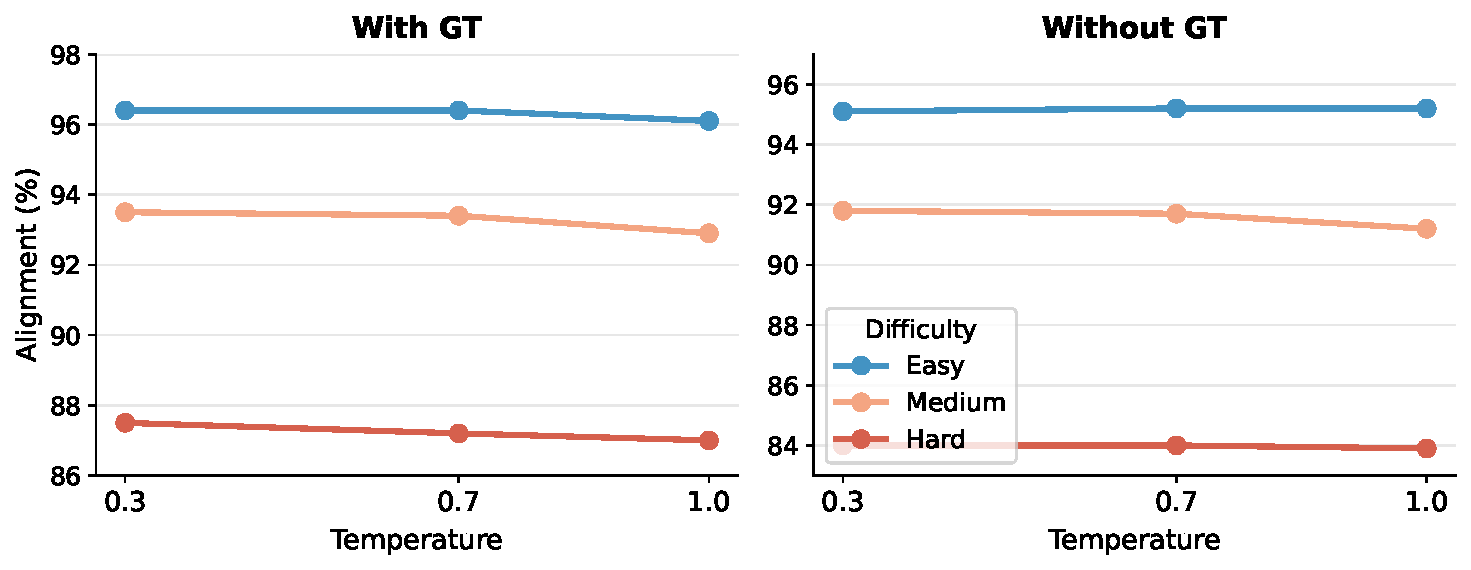
\includegraphics[width=\columnwidth]{figures/abl_temperature.pdf}
\caption{%
\textbf{Judge temperature sensitivity.}
Qwen3-32B alignment at $T \in \{0.3, 0.7, 1.0\}$ on Llama-3.3-70B.
All three difficulty curves are near-flat; maximum spread $\leq 0.6$\,pp.}
\label{fig:abl-temperature}
\end{figure}

\begin{figure}[h!]
\centering
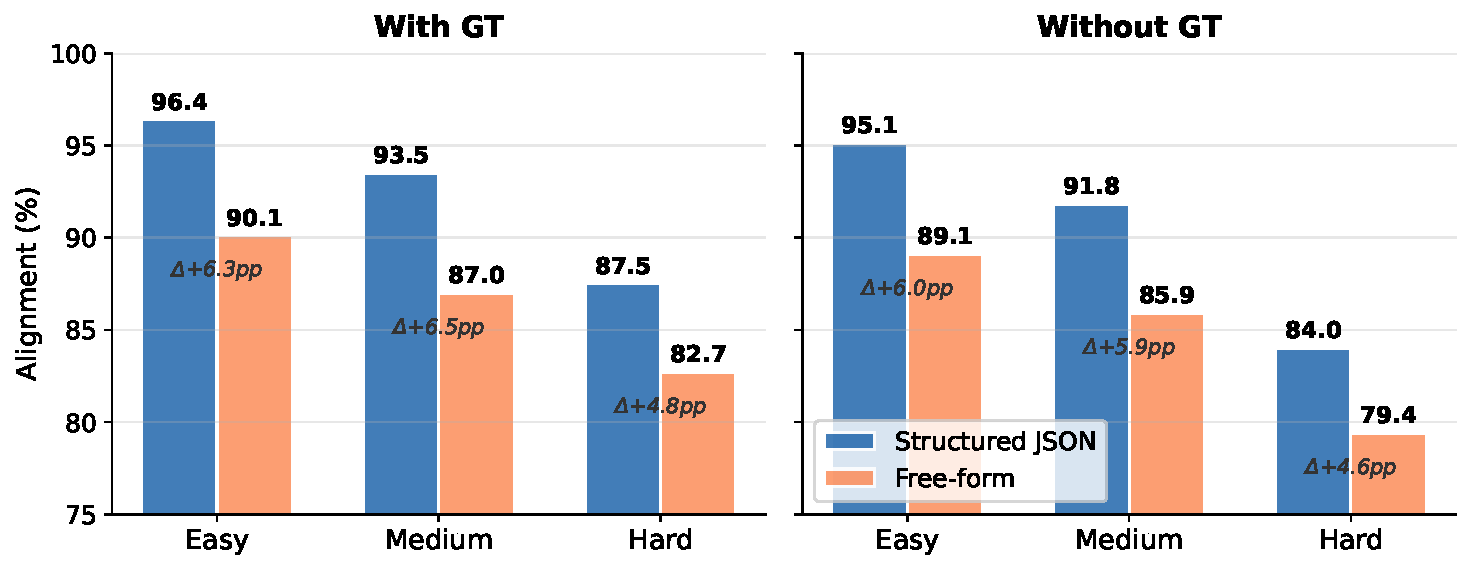
\includegraphics[width=\columnwidth]{figures/abl_format.pdf}
\caption{%
\textbf{Prompt structure vs.\ alignment.}
Structured JSON prompt vs.\ free-form for Qwen3-32B on Llama-3.3-70B.
The per-metric rubric adds $+4.8$-$+6.5$\,pp with GT across all difficulty levels.}
\label{fig:abl-format}
\end{figure}

\textbf{RQ5: Does chain-of-thought reasoning in the judge improve alignment?}
\label{sec:abl:reasoning}

Table~\ref{tab:abl-reasoning} reports QwQ-32B alignment with thinking on vs.\ off across four open-weight generators and three difficulty levels (24 paired cells). CoT reasoning contributes negligibly, with a mean GT gap of $+0.11$\,pp and a maximum per-cell difference of $0.3$\,pp; no cell exceeds $0.3$\,pp on either condition. QwQ-32B's advantage in the main results therefore reflects training distribution rather than inference-time compute. The full per-generator grid is reproduced in Appendix~\ref{app:ablations}.

\begin{table}[t]
\centering
\small
\setlength{\tabcolsep}{3.5pt}
\renewcommand{\arraystretch}{1.02}

\resizebox{\columnwidth}{!}{%
\begin{tabular}{llcccccc}
\toprule

& &
\multicolumn{2}{c}{\textbf{Easy}} &
\multicolumn{2}{c}{\textbf{Medium}} &
\multicolumn{2}{c}{\textbf{Hard}} \\

\cmidrule(lr){3-4}
\cmidrule(lr){5-6}
\cmidrule(lr){7-8}

\textbf{Generator} &
\textbf{Setting} &
\textbf{GT} &
\textbf{No GT} &
\textbf{GT} &
\textbf{No GT} &
\textbf{GT} &
\textbf{No GT} \\

\midrule

\multirow{3}{*}{Llama-3.3-70B}
& Thinking on
  & 96.6 & 95.6 & 93.6 & 92.1 & 87.5 & 84.4 \\
& Thinking off
  & 96.5 & 95.6 & 93.6 & 92.0 & 87.3 & 84.4 \\
& $\Delta$
  & $+0.1$ & $0.0$ & $0.0$ & $+0.1$ & $+0.2$ & $0.0$ \\

\addlinespace[1.5pt]

\multirow{3}{*}{Llama-3.1-8B}
& Thinking on
  & 94.2 & 91.2 & 90.8 & 86.8 & 84.1 & 76.6 \\
& Thinking off
  & 94.3 & 91.4 & 90.8 & 86.8 & 83.9 & 76.7 \\
& $\Delta$
  & $-0.1$ & $-0.2$ & $0.0$ & $0.0$ & $+0.2$ & $-0.1$ \\

\addlinespace[1.5pt]

\multirow{3}{*}{Qwen3-32B}
& Thinking on
  & 95.0 & 93.9 & 90.9 & 89.1 & 84.7 & 81.1 \\
& Thinking off
  & 94.9 & 94.0 & 90.8 & 89.0 & 84.7 & 81.1 \\
& $\Delta$
  & $+0.1$ & $-0.1$ & $+0.1$ & $+0.1$ & $0.0$ & $0.0$ \\

\addlinespace[1.5pt]

\multirow{3}{*}{SmolLM3-3B}
& Thinking on
  & 90.0 & 86.7 & 84.8 & 80.3 & 77.2 & 69.7 \\
& Thinking off
  & 89.8 & 86.7 & 84.6 & 80.4 & 76.9 & 69.7 \\
& $\Delta$
  & $+0.2$ & $0.0$ & $+0.2$ & $-0.1$ & $+0.3$ & $0.0$ \\

\bottomrule
\end{tabular}%
}

\caption{Chain-of-thought reasoning in the QwQ-32B judge: alignment (\%) with thinking on vs.\ off across four open-weight generators. $\Delta$ = thinking-on $-$ thinking-off (pp).}
\label{tab:abl-reasoning}

\end{table}

\textbf{RQ6: Does prompt output format affect alignment?}
\label{sec:abl:format}

Figure~\ref{fig:abl-format} shows that the structured per-metric JSON prompt (verbatim in Appendix~\ref{app:prompt-gt}/\ref{app:prompt-without GT}) outperforms a free-form variant (Appendix~\ref{app:prompt-freeform}) by $+4.8$--$+6.5$\,pp with GT across all difficulty levels on the original (Qwen3-32B, Llama-3.3-70B) pairing, the largest lever we test among the configuration choices in this study. A second pairing (QwQ-32B on SmolLM3-3B) partially replicates this: structured format still wins on easy ($+3.9$\,pp) and medium ($+2.4$\,pp), but the effect shrinks relative to the first pairing and \emph{reverses} on hard ($-0.8$\,pp, free-form marginally ahead). We therefore do not treat prompt format as a uniformly dominant, difficulty-independent lever: the effect is real and judge/generator-dependent, largest on easier queries, and not guaranteed to generalise in direction on hard queries for every pairing. Full tables for both pairings are in Appendix~\ref{app:ablations}.